\documentclass[thesis.tex]{subfiles}
\newcommand\TPR{\mathit{TPR}}
\newcommand\FPR{\mathit{FPR}}
\newcommand\Prec{\mathit{P}}
\newcommand\OMP{\mathit{1-P}}
\newcommand\TP{\mathit{TP}}
\newcommand\FP{\mathit{FP}}
\newcommand\TN{\mathit{TN}}
\newcommand\FN{\mathit{FN}}
\def\x{\mathbf{x}}
\begin{document}

\chapter{Methods}
In this chapter we will go through basic computer vision theory and methods that we have found relevant throughout our work.
\todo{Add proper introduction to the chapter once it's finished}

\section{Gaussian scale-space}
\label{sec:GaussianScaleSpace}
%
When taking pictures of the real world, the resulting images are of various sizes and resolutions, and include objects at different distances. This causes details to be present in the images at various scales. Using the Gaussian scale-space representation \cite{griffin1997scale,ginneken2000applications} described in this section, we are able to create a multi-scale representation of the details in an image. The representation consists of a set of smoothed versions of the original image, obtained by applying Gaussian filters $G$ of various sizes $\sigma$ corresponding to the image scales. When an image is smoothed by a filter at scale $\sigma$, the details smaller than that scale are removed. For a point $(x,y)$, the Gaussian filter at scale $\sigma$ is defined as
%
\begin{align}
	G(x,y;\sigma) &= \frac{1}{2\pi \sigma^2} \exp \left(\frac{-(x^2+y^2)}{2\sigma^2} \right)
\end{align}
%
and the corresponding scale-space image $L(x,y;\sigma)$ is defined as
%
\begin{align}
	L(x,y;\sigma) &= G(x,y;\sigma) \ast I(x,y),\hspace{1cm}\sigma > 0
\end{align}
%
where $I(x,y)$ is the intensity of the original image $I$ in $(x,y)$ and $\ast$ denotes the convolution operator defined as
\begin{align*}
	f(x,y) \ast g(x,y) &= \int\limits_{\tau_1 = -\infty}^\infty \int\limits_{\tau_2 = -\infty}^\infty f(\tau_1,\tau_2) \cdot g(x-\tau_1,y-\tau_2)\,\text{d}\tau_1\,\text{d}\tau_2
\end{align*}
for the two functions $f$ and $g$ \cite[p.~345]{gonzalez:2008:digital}.

Note that while these scale-space functions are defined on an infinite continuum, in practice we select a finite set of scales for which we wish to retrieve structural information in an image.

\Cref{fig:scaleSpaceExample} shows an example of a finite scale-space representation of an image using the five scales $\sigma = 1,2,4,8,16$. At smaller scales ($\sigma = 1,2$) we are still able to see detailed structure in the gates, pavement, car, hedge, etc. When increasing the scale to $\sigma = 4$, the small details are smoothed out and only the larger details of the mentioned objects are noticeable. At $\sigma = 8, 16$ the details are completely smoothed out and only the larger overall structures are visible. This example clearly shows the power of the scale-space representation being able to model both small details as well as larger structures.
%
\begin{figure}[p]
	\centering
	\begin{subfigure}[t]{0.3\textwidth}
		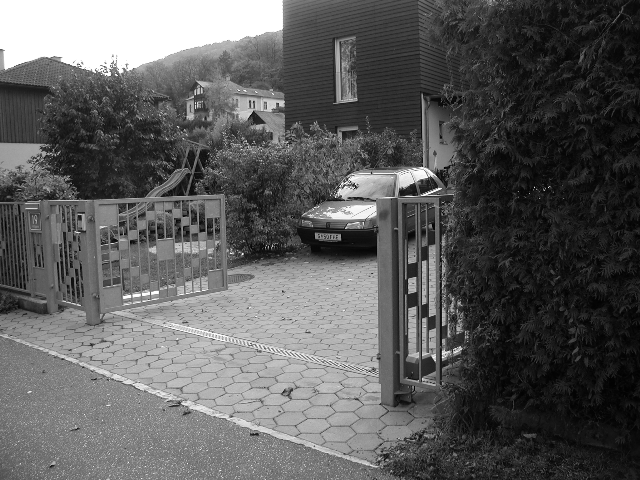
\includegraphics[width=\textwidth]{img/scaleSpaceTheory_0.png}
		\caption{Original}
		\label{fig:scaleSpaceExample0}
	\end{subfigure}
	\begin{subfigure}[t]{0.3\textwidth}
		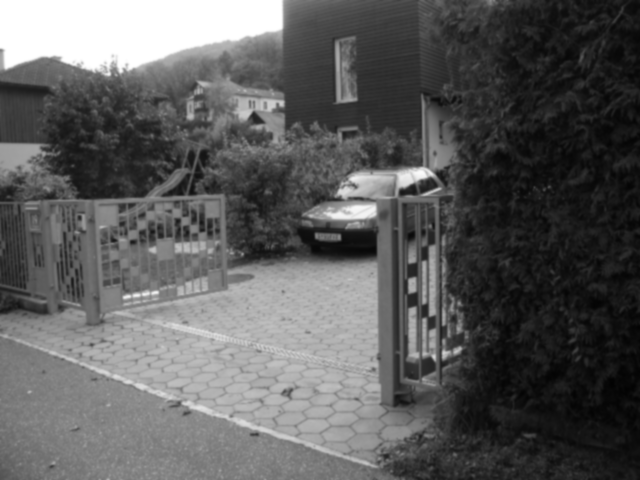
\includegraphics[width=\textwidth]{img/scaleSpaceTheory_1.png}
		\caption{$\sigma = 1$}
		\label{fig:scaleSpaceExample1}
	\end{subfigure}
	\begin{subfigure}[t]{0.3\textwidth}
		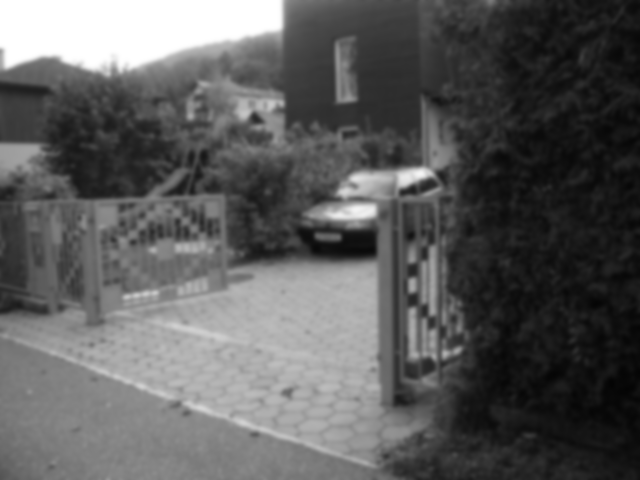
\includegraphics[width=\textwidth]{img/scaleSpaceTheory_2.png}
		\caption{$\sigma = 2$}
		\label{fig:scaleSpaceExample2}
	\end{subfigure}
	\begin{subfigure}[t]{0.3\textwidth}
		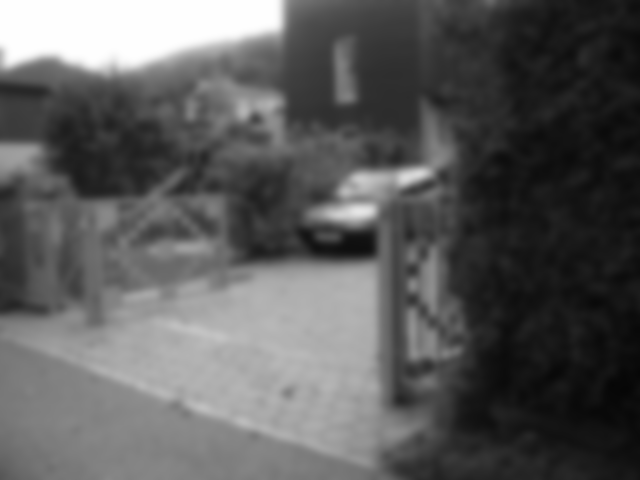
\includegraphics[width=\textwidth]{img/scaleSpaceTheory_4.png}
		\caption{$\sigma = 4$}
		\label{fig:scaleSpaceExample4}
	\end{subfigure}
	\begin{subfigure}[t]{0.3\textwidth}
		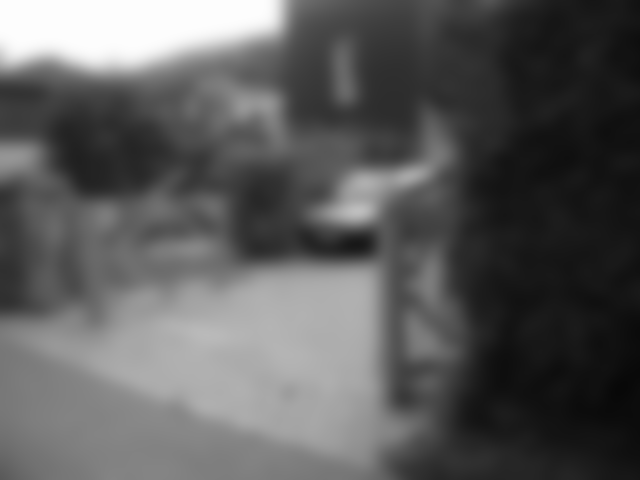
\includegraphics[width=\textwidth]{img/scaleSpaceTheory_8.png}
		\caption{$\sigma = 8$}
		\label{fig:scaleSpaceExample8}
	\end{subfigure}
	\begin{subfigure}[t]{0.3\textwidth}
		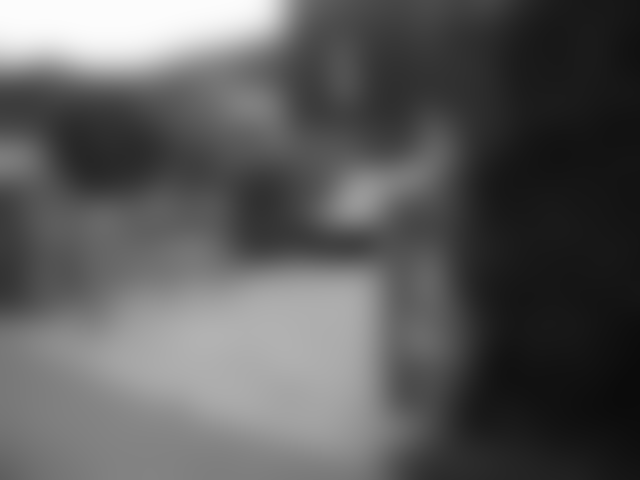
\includegraphics[width=\textwidth]{img/scaleSpaceTheory_16.png}
		\caption{$\sigma = 16$}
		\label{fig:scaleSpaceExample16}
	\end{subfigure}
	\caption{Example of a finite scale-space representation with scales $\sigma = 1,2,4,8,16$ of an image from the INRIA dataset (\Cref{sec:odDataset}).}
	\label{fig:scaleSpaceExample}
	\vspace{0.5cm}
	
	\begin{subfigure}[t]{0.23\textwidth}
		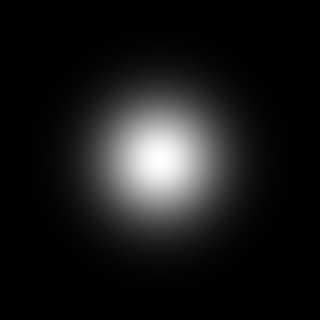
\includegraphics[width=\textwidth]{img/gaussianDerivative_0_0.png}
		\caption*{$G$}
	\end{subfigure}
	\vspace{2mm}	
	
	\begin{subfigure}[t]{0.23\textwidth}
		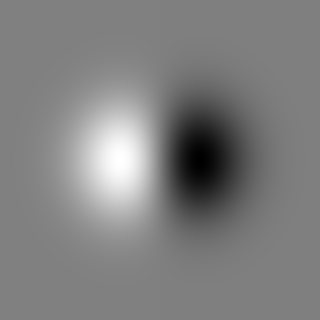
\includegraphics[width=\textwidth]{img/gaussianDerivative_1_0.png}
		\caption*{$G_{x}$}
	\end{subfigure}
	\begin{subfigure}[t]{0.23\textwidth}
		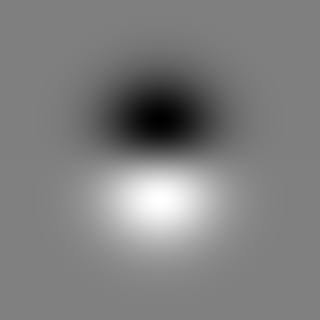
\includegraphics[width=\textwidth]{img/gaussianDerivative_0_1.png}
		\caption*{$G_{y}$}
	\end{subfigure}
	\vspace{2mm}
	
	\begin{subfigure}[t]{0.23\textwidth}
		
\includegraphics[width=\textwidth]{img/gaussianDerivative_2_0.png}
		\caption*{$G_{xx}$}
	\end{subfigure}
	\begin{subfigure}[t]{0.23\textwidth}
		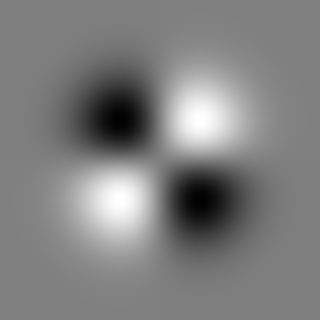
\includegraphics[width=\textwidth]{img/gaussianDerivative_1_1.png}
		\caption*{$G_{x y}$}
	\end{subfigure}
	\begin{subfigure}[t]{0.23\textwidth}
		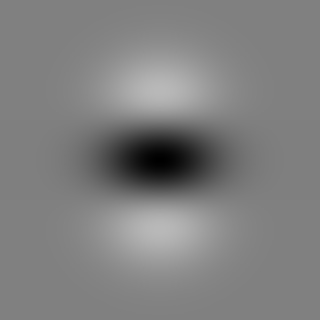
\includegraphics[width=\textwidth]{img/gaussianDerivative_0_2.png}
		\caption*{$G_{yy}$}
	\end{subfigure}
	\caption{Gaussian derivatives up to second order.}
	\label{fig:gaussianDerivatives}
\end{figure}

\section{Differential structure}
\label{sec:diffStructure}
When analysing an image, we are usually interested in the structure of the image. A typical approach to describing the structure is to compute the derivatives of the image up to the n'th order. Real world images are however usually filled with small-grained noise, which is why we often prefer to combine the derivative calculations with a smoothing of the image using a Gaussian filter. The details of this step are explained further in \Cref{sec:gaussianDerivatives}. The first order information, called the gradient, is described in \Cref{sec:gradientTheory}, and the second order information in the form of the shape index is described in \Cref{sec:shapeIndexTheory}.

\subsection{Gaussian derivatives}
\label{sec:gaussianDerivatives}

The \emph{Gaussian derivatives} $G_{x^m y^n}$, where $m$ and $n$ are the order of derivations with respect to $x$ and $y$, are used for obtaining structural information from an image. \Cref{fig:gaussianDerivatives} illustrates the Gaussian derivatives up to second order.

Based on the Gaussian derivatives we define the Gaussian derivative scale-space images $L_{x^m y^n}$:
\begin{align}
	L_{x^m y^n}(x,y;\sigma) &= G_{x^m y^n}(x,y;\sigma) \ast I(x,y)
\end{align}
%
The complexity of the convolution is not irrelevant when calculating scale spaces. Given a filter $f$ with $k$ elements and an image $I$ with $l$ entries, the complexity of a convolution is $\mathcal{O}(k l)$ since we perform $k$ multiplications and $k-1$ summations for each of the $l$ elements. Here we have assumed that the boundaries of the image are padded to allow a full filter computation for all $l$ entries.
In theory the Gaussian function has infinite support causing the Gaussian filter to be infeasibly large. In practice one often uses the 3-sigma rule to determine the support radius of the Gaussian filter and hence the computational load of the convolution. The rule states that approximately 99.7\% of the area under a Gaussian function lies within 3$\sigma$ of the center of the function, and hence using $3\sigma$ as the Gaussian function support radius suffices.

When computing a single Gaussian derivative image, a typical approach is to solve $G_{x^m y^n}$ analytically and sample the 2D filter from the analytical solution. Given a square filter of width and height $6\sigma$ we get $k=(6\sigma)^2$ filter elements. By solving $G_{x^m}$ and $G_{y^n}$ analytically, sampling two 1D filters of size $6\sigma$ and performing two chained convolutions of $I$, we get the same resulting image but at the cost of two significantly smaller filter convolutions. The same strategy can of course be applied to other separable 2D filters such as the ordinary Gaussian smoothing filter.

Since the Gaussian derivative scale-spaces are computed on a set of increasing scales, we need to compute all the needed derivatives for each scale. This give us a large amount of convolutions of the same image using various sizes Gaussian filters, which is computationally inefficient. Given these circumstances, we now describe an alternative and computationally cheaper way of computing the Gaussian derivative scale-spaces. The idea is to compute one smoothing per scale, and then calculate all the derivatives at that scale using finite differences filters. We first define the central differences filter $f$:
%
\begin{align*}
	I_x &= \frac{\partial I}{\partial x} \approx f_x \ast I = \begin{bmatrix} -1 & 0 & 1\end{bmatrix} \ast I \\
	I_y &= \frac{\partial I}{\partial y} \approx f_y \ast I = \begin{bmatrix} -1 & 0 & 1\end{bmatrix}^\text{T} \ast I
\end{align*}
%
The $f_{x^m}$ filter is made by convolving $m$ $f_x$-filters in a chain and the $f_{y^n}$-filter is constructed similarly. The combined derivative is calculated by following the alternative approach above, where we chain two 1D convolutions of $G$ together:
%
\begin{align*}
	L_{x^m y^n}(x,y;\sigma) &= G_{x^m y^n}(x,y;\sigma) \ast I(x,y) \\
		&\approx f_{x^m} \ast \left( f_{y^n} \ast \left (G(x,y;\sigma) \ast I(x,y) \right) \right) \\
		&= f_{x^m} \ast \left( f_{y^n} \ast L(x,y;\sigma) \right)
\end{align*}
%
Since we have a nice set of increasing scales for our scale-space images, we are able to compute $L(x,y,\sigma_2)$ by using the previous scale space $L(x,y,\sigma_1)$ where $\sigma_2 > \sigma_1$ as described in \cite{tola2008fast}. The idea is to split up the smoothing into two operations and then use the associativity of convolution to use the previous scale-space image for the new smoothing:
%
\begin{align*}
	L(x,y;\sigma_2) &= G(x,y;\sigma_2) \ast I(x,y) \\
					&= (G(x,y;\sigma_\Delta) \ast G(x,y;\sigma_1)) \ast I(x,y),\hspace{1cm}\sigma_2 > \sigma_1 \\
					&= G(x,y;\sigma_\Delta) \ast L(x,y;\sigma_1) \\
			 \sigma_\Delta &= \sqrt{\sigma_2^2 - \sigma_1^2}
\end{align*}
%
Which give us the final equations for the alternative way of computing the Gaussian derivative scale-spaces.

\subsection{Gradient orientation and magnitude}
\label{sec:gradientTheory}
%
The \emph{gradient orientation} $\Theta \in [-\pi,\pi]$ is the orientation of the local first order derivatives. $\Theta$ is independent of the size of the derivatives, which is given by the \emph{gradient magnitudes} $M$. $\Theta$ and $M$ are defined in terms of the image derivatives as
%
\begin{align*}
\Theta &= \text{atan2}(L_y,L_x) \\
M &= \sqrt{L_x^2 + L_y^2}
\end{align*}
where atan2 is the arctangent function spanning the whole range of angles $[-\pi,\pi]$.
%
\Cref{fig:gradientOrientationTheory} illustrates the relationship between the gradient orientation, gradient magnitude, and $x$- and $y$-derivatives.
%
\begin{figure}[p]
	\centering
	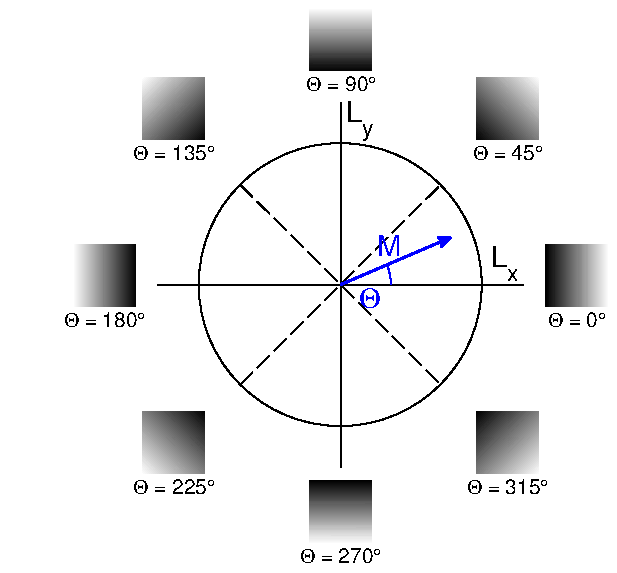
\includegraphics[width=0.63\textwidth,clip=true,trim=31 0 0 0]{img/gradientOrientationTheory.pdf}
	\caption{Gradient orientation and magnitude shown in the coordinate system $(L_x,L_y)$ of first order image derivatives.}
	\label{fig:gradientOrientationTheory}
	\vspace{0.5cm}	
	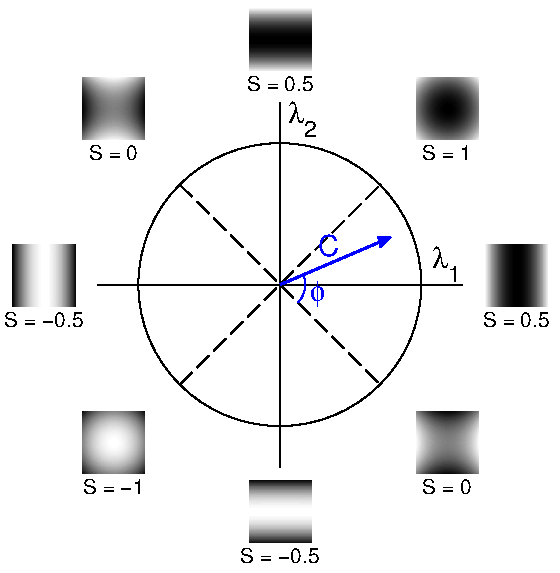
\includegraphics[width=0.63\textwidth,clip=true,trim=31 0 0 0]{img/shapeIndexTheory.pdf}
	\caption{Shape index and curvedness shown in the coordinate system $(\kappa_1,\kappa_2)$ of principal curvatures. The blue vector illustrates a shape index $S = \frac{2}{\pi} \phi$ and curvedness $C$, where $\phi$ is the signed angle between the vector and the line $\kappa_2 = -\kappa_1$. Note that the order of $\kappa_1$ and $\kappa_2$ does not matter, as shape index is independent of the orientation of the local geometry.}
	\label{fig:shapeIndexTheory}
\end{figure}

\subsection{Shape index and curvedness}
\label{sec:shapeIndexTheory}
%
The \emph{shape index} $S \in [-1,1]$ \cite{koenderink1992surface} is a scalar characterization of local second order derivatives. Like $\Theta$ and $M$, $S$ is independent of the size of the derivatives, which is given by the \emph{curvedness} $C$. Additionally the shape index is independent of orientation.

$S$ is defined by the orientation of the eigenvalues $\kappa_1$ and $\kappa_2$, also called the principal curvatures, of the local Hessian matrix $\nabla^2 L$. It can also be expressed by the local image derivatives:
%
\begin{align}
S &= \frac{2}{\pi} \Atan{\frac{\kappa_1 + \kappa_2}{\kappa_1 - \kappa_2}} \\
&= \frac{2}{\pi} \Atan{\frac{-L_{xx} - L_{yy}}{\sqrt{4 L_{xy}^2 + (L_{xx} - L_{yy})^2}}}
\end{align}
%
$C$ is defined by the size of $\kappa_1$ and $\kappa_2$, and can also be expressed by the image derivatives:
%
\begin{align}
C &= \sqrt{\frac{\kappa_1^2 + \kappa_2^2}{2}} \\
&= \frac{1}{\sqrt2} \sqrt{L_{xx}^2 + 2 L_{xy}^2 + L_{yy}^2}
\end{align}
%
\Cref{fig:shapeIndexTheory} illustrates the relationship between the principal curvatures, shape index and curvedness, as well as the geometry of various shape indices. As seen in the figure, $S$ ranges over light blobs ($S = -1$), ridges ($S = -0.5$), saddle points ($S = 0$), valleys ($S = 0.5$), and dark blobs ($S = 1$) with continuous deformations in between.
%
\section{Histograms}
\label{sec:histograms}

Histograms play an essential role in SIFT-like descriptors. They are used for aggregating gradient orientation (GO) and magnitude information over local areas. Traditionally histograms have been constructed using hard boundaries between bins; and descriptors have been constructed with hard boundaries between the local histogram areas of a descriptor.

These types of histograms are however neither robust to small interest point translation/detection errors or gradient orientations close to the bin boundaries. SIFT used a trilinear interpolation of the gradient magnitude based on the radial distance between the gradient orientation and the bin centers to cope with gradients close to the bin boundaries. In order to improve upon the robustness of the histograms, we here describe a histogram framework which is able to produce both ordinary (hard bounded) as well as smooth histograms based on locally orderless images (LOI), \cite{koenderink1999structure}.

The idea behind smooth histograms is to remove the sharp boundaries of ordinary histograms (bin boundaries). Given a position we wish to create a histogram for the surrounding local area/region of interest (ROI). This is done by letting all the values from the ROI contibute to all the bins of the histogram. When looking at discrete problems, this corresponds to using a Parzen window technique \cite{parzen1962estimation}. \mycomment[MSN]{Should this be mentioned or not?}

Given a value function $f$ with a range of $[f_\text{min},f_\text{max}]$, and a spatial ROI center $\x_0$, we wish to compute the histogram $H$ value at bin center $f_i$.
The value function defined as $f(\x,\sigma)$ corresponds to calculating the function $f$ in position $\x$ at (inner) scale $\sigma$. In terms of images this could correspond to calculating the gradient orientation at a position $\x$ in a scale space image at scale $\sigma$.
We use the distance between the bin center $f_i$ and $f(\x,\sigma)$ to compute the bin aperture function $B$ using the (tonal) scale $\beta$ as ``width'' of $B$. Finally we compute a spatial aperture function $A$ of the distance between $\x_0$ and $\x$ using the (outer) scale $\alpha$ as the ``width'' of $A$. The histogram of the bin center $f_i$ is defined from $f,~B,$ and $A$ as
%
\begin{align}
	\label{eq:histogramLong}
	H(f_i;\x_0,\sigma,\beta,\alpha) &= \int A(\x;\x_0,\alpha) B(f(\x;\sigma)-f_i;\beta)\,\text{d}\x
\end{align}
%
When using such a histogram in practice, the parameters $\x_0,~\sigma,~\beta,$ and $\alpha$ are already defined as well as the functions $A,~B,$ and $f$ leading to the following shorthand notation for a histogram:
%
\begin{align}
	\label{eq:histogramShort}
	H(f_i) &= \int A(\x) B(\x;f_i,f)\,\text{d}\x
\end{align}
%
The specifics of the histograms used in our work are explained in \Cref{eq:proposed_histogram}.
%
\subsection{Aperture kernel functions}
\label{sec:apertureKernelFunctions}
%
We consider three choices of kernel functions for $A$ and $B$: box, triangle, and Gaussian. In 1D, the kernels are defined as
%
\begin{align*}
\mathit{Box} (x; \beta) &= 
\begin{cases}
    \frac{1}{2 \beta},& \text{if } |x| \leq \beta \\
    0,              & \text{otherwise}
\end{cases} \\
\mathit{Tri} (x; \beta) &= 
\begin{cases}
    \frac{1}{2 \beta} \left( 1 - \frac{| x |}{2 \beta} \right) ,& \text{if } |x| \leq 2 \beta \\
    0,              & \text{otherwise}
\end{cases} \\
G(x;\beta) &= \frac{1}{\sqrt{2\pi} \beta}
\exp\left( -\frac{x^2}{2 \beta^2} \right)
\end{align*}
%
For bin aperture functions $B$ we can use these kernels directly. The spatial aperture functions $A$ are however defined on a 2D domain; this is handled by multiplying two of the same kernel functions together, e.g:
%
\begin{align*}
G(\x;\alpha) &= G(x;\alpha) G(y;\alpha) \\
&= \frac{1}{2\pi \alpha^2}
\exp\left( -\frac{x^2 + y^2}{2 \alpha^2} \right)
\end{align*}
%
where $\x = [x ~~ y]^T$. We do not allow for separate scales $\alpha$ for each dimension.
%
\subsection{Periodic histograms}
When creating histograms of periodic domains $[f_\text{min}, f_\text{max}]$, we need to take the periodicity into consideration.
The periodicity of the domain means that there are multiple distances between any two points. Since we are computing distance bin aperture functions, we need to find the minimum distance $d_{wrap}$ from each point value to each bin center in order to correctly compute the function values. This is done by a simple wrap-around using the known period of the domain as maximum distance:
\begin{align*}
	d_{wrap} = \min(d,(f_\text{max} - f_\text{min})-d)
\end{align*}
where $d$ is the distance $x - \mu$ from a point $x$ to a bin center $\mu$, and $\min$ is the function that chooses the lowest of its arguments.

 \Cref{fig:1dFilterGaussianPeriodic,fig:1dFilterTrianglePeriodic,fig:1dFilterBoxPeriodic} show 1D examples of four periodic Gaussian, triangle and box kernels respectively on the interval $[-1,1]$. Notice how the wrap-around affects the kernels at both ends of the periods.

\subsection{Renormalization}
When making histograms over a non-periodic domain, the weight function will be cropped by the histogram bounds $f_\text{min}$ and $f_\text{max}$. We therefore risk biasing the weights towards the central bins of the domain, since the cropped filters will have. In order to avoid this, we view the bins as probability densities, and hence the area under each bin's weight function has to integrate to 1. This is done by renormalizing the functions based on their areas. Given a bin aperture function $B$ and a bin center $f_i$, for which $f_\text{min} \leq f_i \leq f_\text{max}$ we calculate the bounds $a$ and $b$ when $B$ is centered around $f_i$:
\begin{align*}
	a = f_\text{min} - f_i,\hspace{1cm}
	b = f_\text{max} - f_i,\hspace{1cm}
\end{align*}
We notice that $a \leq 0 \leq b$. The renormalized bin aperture function $B_\text{renorm}$ is obtained by dividing $B$ with its definite integral:
\begin{align*}
	B_\text{renorm}\left( f(\x;\sigma)-f_i;\beta \right) = \frac{B \left(f(\x;\sigma)-f_i;\beta \right)}{\int_a^b B \left( z;\beta \right)\,\text{d}z}
\end{align*}
Notice how the bounds $a$ and $b$ of the integral are offset by the bin center $f_i$. The definite integrals of our chosen kernel functions are computed in \Cref{apx:histogramRenormalization}.

\Cref{fig:1dFilterGaussianRenorm,fig:1dFilterTriangleRenorm,fig:1dFilterBoxRenorm} show 1D examples of four renormalized Gaussian, triangle, and box filters respectively on the interval $[-1,1]$. Notice how the two weight functions of the outer-most bins have higher peaks than the central bins in order to integrate to 1 when being cut off at the interval bounds. For periodic histograms the renormalization step is excluded since no cut off of the filters occurs.
\todo{Decide what to do with the poor box illustration}

\begin{figure}
	\centering
	\begin{subfigure}[t]{0.32\textwidth}
		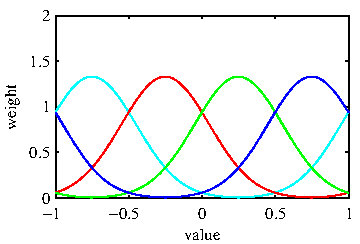
\includegraphics[width=\textwidth]{img/binFilterGaussianPeriodic.pdf}
		\caption{Periodic Gaussian}
		\label{fig:1dFilterGaussianPeriodic}
	\end{subfigure}
	\begin{subfigure}[t]{0.32\textwidth}
		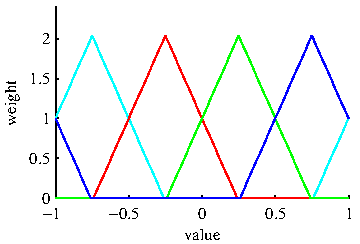
\includegraphics[width=\textwidth]{img/binFilterTrianglePeriodic.pdf}
		\caption{Periodic triangle}
		\label{fig:1dFilterTrianglePeriodic}
	\end{subfigure}
	\begin{subfigure}[t]{0.32\textwidth}
		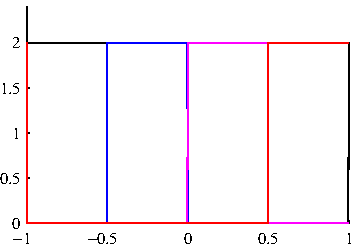
\includegraphics[width=\textwidth]{img/binFilterBoxPeriodic.pdf}
		\caption{Periodic box}
		\label{fig:1dFilterBoxPeriodic}
	\end{subfigure}
	\begin{subfigure}[t]{0.32\textwidth}
		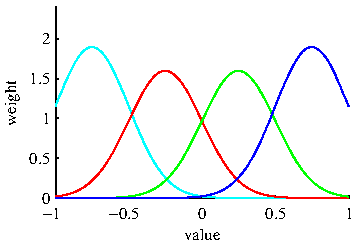
\includegraphics[width=\textwidth]{img/binFilterGaussianRenorm.pdf}
		\caption{Renorm. Gaussian}
		\label{fig:1dFilterGaussianRenorm}
	\end{subfigure}
	\begin{subfigure}[t]{0.32\textwidth}
		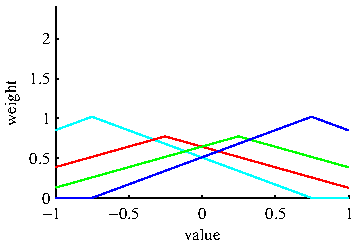
\includegraphics[width=\textwidth]{img/binFilterTriangleRenorm.pdf}
		\caption{Renorm. triangle}
		\label{fig:1dFilterTriangleRenorm}
	\end{subfigure}
	\begin{subfigure}[t]{0.32\textwidth}
		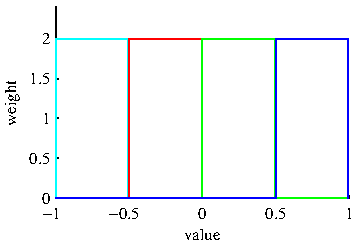
\includegraphics[width=\textwidth]{img/binFilterBoxRenorm.pdf}
		\caption{Renorm. box}
		\label{fig:1dFilterBoxRenorm}
	\end{subfigure}
	\caption{Examples of periodic and renormalized 1D Gaussian, triangle, and box functions. Each figures contains four filters centered at values $-0.75$, $-0.25$, $0.25$, and $0.75$ and with $\sigma = \nicefrac{1}{2}$.}
	\label{fig:1dFilters}
\end{figure}
%
\section{Invariants and robustness}
When describing interest points and their local regions in real world images, we experience a lot of transformations of the actual physical objects. We are however interested in being able to describe the interest point without any (or a predefined set) of these transformations applied, in which case we have a better chance of recognizing the interest point in other images.

Apart from invariance to various transformations we also want to be robust to small changes in some of the transformations. This robustness should give us nearly equal descriptors despite having small errors in our estimation of the transformations.
In this section we will go through a list of transformations that we wish for our descriptor to be invariant and possibly also robust to.

\begin{table}[H]
	\centering
	\begin{tabular}{@{}l|ll@{}}
	%\toprule
	Measure & Rotation & Illumination \\
	\hline
	$\Theta$ & $\Theta - \theta $ & $\Theta$ \\
	$M$ & $M$ & $a M$ \\
	$S$ & $S$ & $S$ \\
	$C$ & $C$ & $a C$ \\
	%\bottomrule
	\end{tabular}
	\caption{The transformation of various measures by rotation and illumination. The derivations are included in \cref{apx:image_transformations}.}
	\label{tbl:measureInvariances}
\end{table}

\subsection{Translation}
The first transformation that we describe is translation. Translation occurs when images are taken from different positions and hence the interest points are translated in the image plane. Translation invariance is often achieved by combining a descriptor with an interest point detector which tells the descriptor where the interest points are located spatially in the image. Another approach is to use a sliding window technique in which a detection window is moved around the image trying to find a suitable matching position as in \cite{felzenszwalb2008discriminatively}. Translation invariance is almost always desired since even tiny vibrations at the time of capture can cause an object to change position in an image.

An interest point detector or a sliding window is only able to give an estimate of positions of interest points based on the detail available in the pixels of the image. We therefore also wish to have a descriptor which is robust to small changes in interest point positions allowing for a small error in detection point without having a large impact on the descriptor.

\subsection{Rotation}
Rotation naturally occurs when either the camera or the object in question is rotated. Even though a precise position is located, the outcome of descriptors with spatial pooling will be affected by rotation, if no efford is done to achieve rotational invariance. For SIFT-like descriptors the general approach to achieving rotational invariance is to estimate the direction of the feature and rotate the descriptor grid before computing the descriptor. Rotation invariance is often desired but not always needed, as in \cite{dalal2005histograms,felzenszwalb2008discriminatively} where only detection of pedestrians in upright positions is needed.

Looking at the differential measures $\Theta, M,~S,$ and $C$, we are able to derive the resulting measure under rotation by $\theta$. We have left out the details of the derivations here, but they can be found in \Cref{apx:rotation}. The final derived results are shown in \Cref{tbl:measureInvariances}. We see that both $M,~S,$ and $C$ are rotational invariant whereas $\Theta$ is rotated by the transformation angle $\theta$.
%
\subsection{Reflection}
Reflection occurs when either an object is flipped along some axis or an entire image is flipped (typically along the x- and/or y-axis). An example could be two sideshot images of a car driving in opposite directions, since a car typically looks the same from either side. Reflection is typically not handled directly in the descriptor but rather in the applications of the descriptor. An example of this is the pedestrian detection application, where \cite{dalal2005histograms} make sure to include both the original positive pedestrian images as well as their horizontally flipped versions in order to obtain a more reflection invarian pedestrian detector.

\subsection{Illumination}
\label{sec:illumination}
Illumination transformations both occur as global as well local transformations of light. The global transformation model the overall diffuse light level, which is visible on e.g. a sunny and a cloudy day. The local transformations model the local differences in light such as e.g. cast shadows and directed light.

By assuming the image $\tilde{I} = a I +  b$ is an affine illumination transformation of the underlying image $I$ with no light transformations, we are able to derive the effect of the transformation on the differential measures $\Theta,~M,~S,$ and $C$. Once again we have left out the details here, which can be found in \Cref{apx:illumination}. The final results can be seen in \Cref{tbl:measureInvariances}. We see that $\Theta$ and $S$ are illumination invariant whereas $M$ and $C$ are multiplied by the linear constant $a$ of the affine transformation. These coefficients are typically estimated and corrected for by using some either local or global normalization scheme.

\subsection{Scale}
\label{sec:scaleInvariance}

The scale of objects in images vary depending on multiple factors as descibed in \Cref{sec:GaussianScaleSpace}. In order to achieve scale invariance, descriptors are typically defined relative to a feature scale. Depending on the application, the feature scale is typically defined by an interest point detector or a sliding window.

\subsection{Perspective}
Perspective distortions and occlusions have major impact on images. Even small changes of camera position can distort objects in 2D images and occlusions might occur. The perspective transformations are hard to estimate without prior knowledge of the scene and its attributes. Therefore only perspective robustness to a certain degree has been achieved in descriptors so far.
%
\section{Binary classification measures}
\label{sec:binaryClassificationMeasures}
%
\emph{Binary classification} is the problem of predicting whether elements have one of two conditions: positive ($+1$) or negative ($-1$). Formally, we consider elements $x \in X$ with respective condition labels $y \in \{-1, 1\}$. This is also called the ground truth or golden standard. Without the knowledge of $y$, we wish to assign elements $x \in X$ with a prediction or classification $\hat{y} \in \{-1, 1\}$, ideally equal to $y$.

Many binary classification methods do not directly output such a classification, but rather a more descriptive \emph{classification score} $s \in \mathbb{R}$ for each $x \in X$, that denotes the confidence of a classification. A higher $s$ means that we find it more likely that $x$ has the label $y = 1$. Thus as an intermediate step we can select a threshold $t \in \mathbb{R}$, and classify $x$ with $\hat{y} = 1$ if $s \geq t$, or $\hat{y} = -1$ if $s < t$. Varying this threshold allows us to modify the ratio between elements classified as positive and negative.

To measure the performance of a binary classification method, we could simply compute the ratio of correctly classified elements. However, this measure is flawed if the distribution of elements is skewed toward one of the two conditions, or if it is more important to classify one of the conditions correctly than the other. Instead, we base our measures on the confusion matrix:
%
\begin{table}[H]
	\centering
	\bgroup
	\def\arraystretch{1.5}
	\begin{tabular}{|l|c|c|}
		\cline{2-3}
		\multicolumn{1}{c|}{} & Condition positive & Condition negative \\ \hline
		Assigned positive & \cellcolor{green!25}True Positive (TP) & \cellcolor{red!25}False Negative (FN)  \\ \hline
		Assigned negative & \cellcolor{red!25}False Positive (FP) & \cellcolor{green!25}True Negative (TN) \\ \hline
	\end{tabular}
	\egroup
	\caption{Confusion matrix for binary classification}
	\label{tbl:confusion_matrix}
\end{table}
%
The confusion matrix places classification outcomes into one of four cells, depending on both the condition and assigned label. We define $\TP$, $\FP$, $\FN$, and $\TN$ to be the number of respective outcomes across a given set of elements. We also define the following three measures: \emph{recall} or \emph{true positive rate} ($\TPR$), \emph{fall-out} or \emph{false positive rate} ($\FPR$), and \emph{precision} ($\Prec$):
%
\begin{align*}
	\TPR &= \frac{\TP}{\TP + \FN} \\
	\FPR &= \frac{\FP}{\FP + \TN} \\
	\Prec &= \frac{\TP}{\FP + \TP}
\end{align*}
%
In other words, recall is the percentage of condition positives that we have classified correctly, fall-out is the percentage of condition negatives that we have classified incorrectly, and precision is the percentage of assigned positives that are indeed condition positives.

Recall that these measures depend on the threshold $t$ used for classification. There are two common ways to visualize the effect of $t$: the ROC-curve defined as recall vs. fall-out and the PR-curve defined as precision vs. recall. They are constructed by varying $t$ across $\mathbb{R}$ and plotting the measures as a curve in the respective spaces. A ROC-curve describes the ability to classify both condition positives and negatives correctly, whereas a PR-curve describes the relation between the ``quality'' of assigned positives and the ``quantity'' of assigned condition positives.

In order to get a performance measure independent of the choice of $t$, we can integrate the ROC- and PR-curves giving us the area under the curve (AUC). We refer to these measures as the ROC AUC and PR AUC. The ROC AUC has the property of being the probability that a randomly chosen condition positive element has a higher classification score $s$ than a randomly chosen condition negative element. The PR AUC is also called the average precision, as it is the average precision across all possible recall ratios. \Cref{fig:imageCorrespondenceROC,fig:imageCorrespondencePR} show examples of ROC and PR curves as well as their AUCs for an example of the image correspondence problem.

Note that PR-curves are used when the positive class is the main class of interest, or when a large skew towards one of the conditions of the classification is present as according to \citet{davis2006relationship}. Furthermore \citet{davis2006relationship} prove that an algorithm which optimizes ROC AUC doesn't necessarily optimize PR AUC, and hence optimization algorithms should utilize the final choice of evaluation measure to achieve optimal results. It is however also shown that given two curves, the first curve dominates the second in ROC space if and only if the first curve dominates the second in PR space \cite[Theorem 3.2]{davis2006relationship}, and hence an algorithm which always beats the competitors in PR also beats the competitors in ROC. In this context the notion of a curve dominating another curve means that the second curve is beneath or equal to first (dominating) curve.

The choice between using the ROC- or PR-curves and their AUCs are discussed in the individual application sections \Cref{sec:od,sec:ic}.
%
\section{Welch's $t$-test}
\label{sec:welchsTtest}

Assume we have two sets of samples $X_1$ and $X_2$ from two normal distributions with unequal variances $\sigma_1$ and $\sigma_2$. \emph{Welch's $t$-test} is used for estimating the difference between the two sample means and their distribution intervals. It is defined as
\begin{align*}
	t = \frac{\bar{X_1} - \bar{X_2}}{\sqrt{\frac{s^2_1}{n_1} - \frac{s^2_2}{n_2}}}
\end{align*}
where $\bar{X_1}$ and $\bar{X_2}$ are the means of the samples $X_1$ and $X_2$, $s^2_1$ and $s^2_2$ are the unbiased estimated variances of the samples, and $n_1$ and $n_2$ are the number of samples from each distribution.
\todo{Finish section about Welch's $t$-test}

\section{Interest point detectors}
\label{sec:interestPointDetectors}
As mentioned in \Cref{sec:introduction} interest point detectors are used for finding distinctive points in images having various desired properties. These properties vary between blobs, corners, and edges depending on the detector used. Furthermore some detectors are multi-scale detectors meaning that they search through a scale space pyramid in order to find interest points at multiple scales. Combining a multi-scale detector with a descriptor is a typical way of achieving scale invariant descriptors as mentioned in \Cref{sec:scaleInvariance}.

The focus of this report is to study higher order descriptors and hence we simply choose to use the multi-scale DoG blob detector from SIFT \cite{lowe2004distinctive} described below.

\subsection{Multiscale Difference of Gaussians}
\label{sec:multiscaleDoG}

Recall from \Cref{sec:GaussianScaleSpace} that our scale-space representation removes image details below a given scale $\sigma$. The idea of the Difference of Gaussians (DoG) blob detector is that by computing the difference of two scale-space images for $\sigma_1$ and $\sigma_2$, we also remove the details at a higher scale, leaving only details between $\sigma_1$ and $\sigma_2$. Formally we define
%
\begin{align*}
\Gamma(\x;\sigma_1,\sigma_2) &= L(\x;\sigma_2) - L(\x;\sigma_1) \\
&= \left( G(\x;\sigma_2) - G(\x;\sigma_1) \right) \ast I(\x)
\end{align*}
%
where $\sigma_2 > \sigma_1$. Minima and maxima of this function indicate dark and light blobs, respectively, at a scale between $\sigma_1$ and $\sigma_2$.

In order to create a multi-scale DoG detector, $\Gamma$ is computed across adjacent pairs of scale-space images. In SIFT, the scales are create in scale octaves as illustrated in \Cref{fig:dogSpaces}. When we extract multiscale interest points, we find extremas that are not just extremas in their respective DoG images, but for adjacent DoG images as well. In practice this is done by finding extrema in a 26-pixel neighbourhood. As seen in the illustration, each octave has a number of DoGs, all with the same image size.

The octaves scales are defined as $2^n$ for $n = l,\hdots,h$, where $l$ is the lowest exponent and $h$ is the highest exponent needed for a desired range of octave scales. An octave is split into several scales $s$ (octave resolution), for which we wish to extract interest points. This results in Gaussian images with scale distance $2^{\nicefrac{1}{s}}$ positioned at scales $2^{\nicefrac{m}{s}}$ where $m = l,\hdots,s \cdot h$. The DoGs are however differences of these Gaussians and hence the detection scales are offset in between the Gaussian scales at $2^{\nicefrac{(n+0.5)}{s}}$.
In practice we need to create $s+3$ Gaussian images of the same size for each octave. The first extra Gaussian image ($s+1$) is needed in order to compute the $s$ DoGs. The next two Gaussian images are needed for two additional DoGs surrounding the $s$ initial DoGs, allowing for 26-pixel neighbourhood computations within the entire octave. \Cref{fig:dogSpaces} illustrates this for $s = 2$.

To prevent extracting too many interest points, we can select only the most significant points by placing a threshold on the magnitude of $\Gamma$.

An example of DoG images is shown in \Cref{fig:dogExample}, which is based on the scale-space images from \Cref{fig:scaleSpaceExample}. We see that the two different scales locate dark and light blobs of different sizes. In our work we have been using the VLFeat implementation of the multi-scale DoG detector \citet{vedaldi2008vlfeat}.
%
\begin{figure}[p]
	\centering
	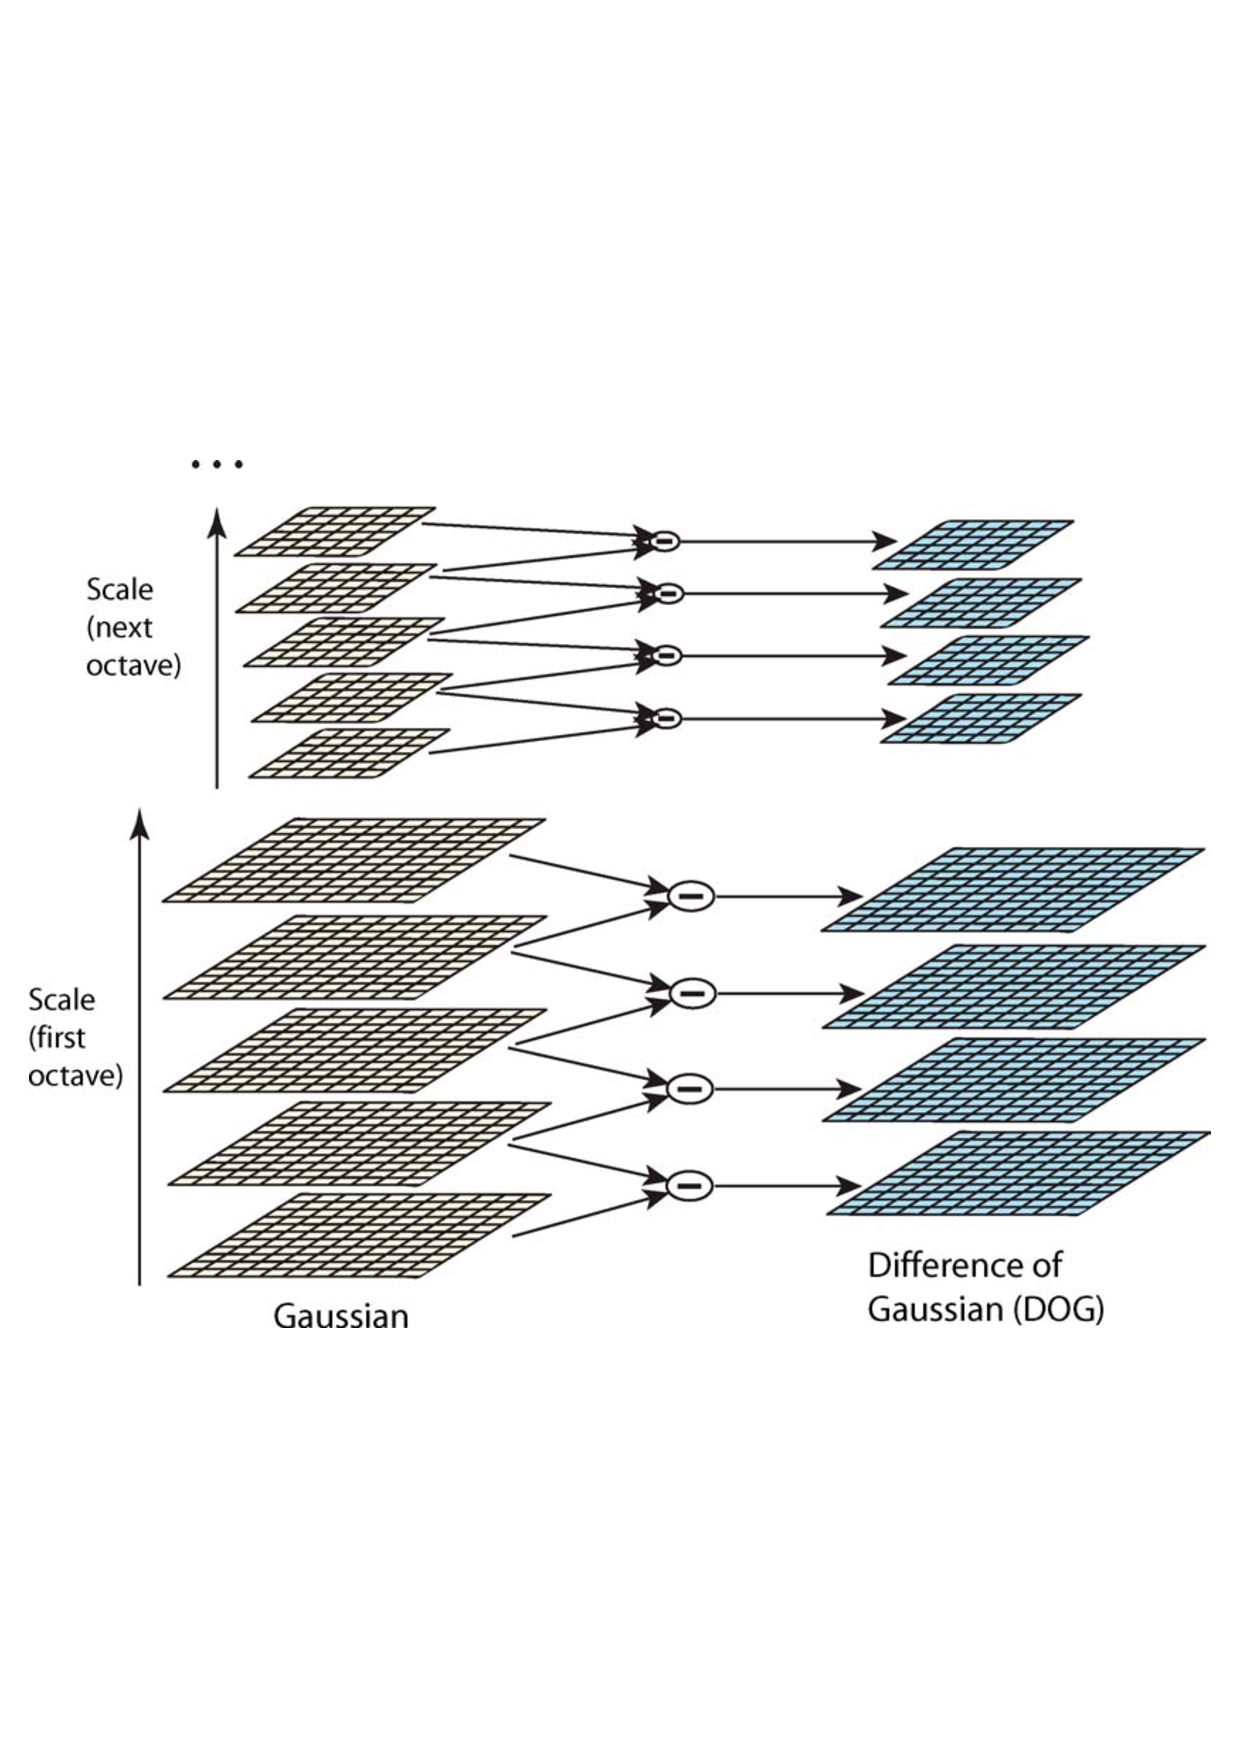
\includegraphics[width=\textwidth,clip=true,trim=0 200 0 220]{img/SIFT_dogspaces.pdf}
	\caption{Illustration of how DoG images are computed by subtracting adjacent Gaussian scale-space images. The resulting images contain details between the two respective scales. This figure is taken from \citet[figure 1,pp. 95]{lowe2004distinctive}.}
	\label{fig:dogSpaces}
	\vspace{5mm}

	\centering
	\begin{subfigure}[t]{0.49\textwidth}
		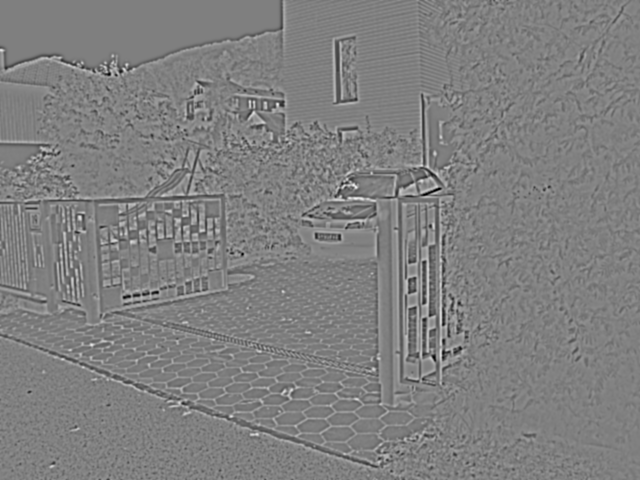
\includegraphics[width=\textwidth]{img/scaleSpaceTheory_2-1.png}
		\caption{$\sigma_1 = 1, \sigma_2 = 2$}
		\label{fig:dogExampleFirst}
	\end{subfigure}
	\begin{subfigure}[t]{0.49\textwidth}
		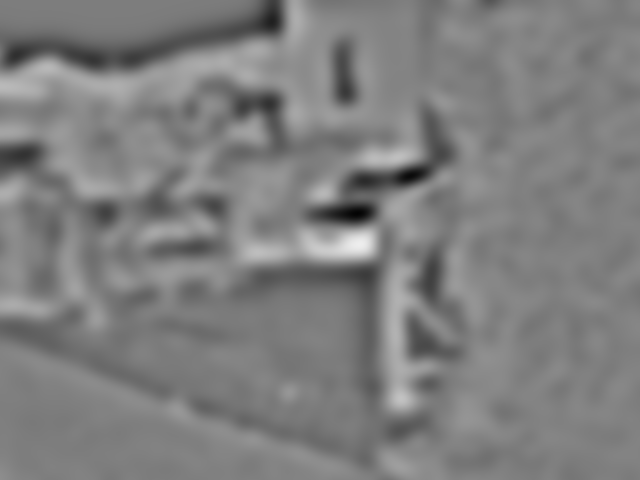
\includegraphics[width=\textwidth]{img/scaleSpaceTheory_16-8.png}
		\caption{$\sigma_1 = 8, \sigma_2 = 16$}
		\label{fig:dogExampleLast}
	\end{subfigure}
	\caption{Example of DoG images computed for the set of scale-space images from \Cref{fig:scaleSpaceExample} at two fine scales $\sigma_1 = 1, \sigma_2 = 2$ and two course scales $\sigma_1 = 8, \sigma_2 = 16$. Light and dark areas correspond to dark and light blobs in the respective scale intervals.}
	\label{fig:dogExample}
\end{figure}

\section{Sliding window}
\label{sec:slidingWindow}
%
Sliding windows are an alternative approach to selecting image regions for which to compute descriptors. Instead of centering regions around interest points, we systematically extract regions from varying positions and scales. Generally this is achieved by placing a square grid in each scale-space image. Regions are then extracted around each grid point at a size respective to each scale. We use a somewhat dense grid, causing a large overlap between regions. The sliding window method is used when we require an exhaustive search of an image, which is the case for object detection.

\section{Descriptors}

The field of descriptors and their applications is wide, and hence we have chosen a descriptor for each of our applications to compare our performance against. In this section we will go through the methods of computing the SIFT and HOG descriptors, which were introduced in the literature study and have proven to perform well on our applications.

\subsection{SIFT}

We shortly described the SIFT descriptor in the literature study. Here we will explain the details of the descriptor.

SIFT utilizes gradient information on grayscale images to compute distinctive interest point descriptors. SIFT was originally proposed in combination with the multi-scale DoG detector described in \Cref{sec:multiscaleDoG}. Apart from the DoG detection steps, the algorithm first determines the orientations of the interest point in question. This is done by computing gradient magnitudes and orientations for a local area around the interest point in the associated scale-space image $L$. From the orientations a histogram of 36 bins is created, where each orientation is weighted by its magnitude and scaled by a Gaussian weight computed from the distance to the interest point. This Gaussian window has $\sigma$ equal to $1.5$ times the detection scale $\sigma_0$. A descriptor is created for the highest peak of the histogram as well as for each of the peaks that have a weight within 80\% of the maximum histogram weight. Finally, the chosen orientations are refined by fitting of a parabola to the three points around each orientation.

Having determined the orientation of an interest point, the local area surrounding the interest point is divided into a grid of $4 \times 4$ cells, each spanning $4 \times 4$ pixels in the $\sigma_0$ scale-space image. For each of these cells a gradient orientation histogram with 8 bins is created. Each sample is weighted by its gradient magnitude. The magnitude is however subject to a trilinear interpolation between adjacent cell- and bin centers. Furthermore all magnitudes are multiplied by a Gaussian window centered at the interest point and having $\sigma$ half the width of the descriptor window.

Once the histograms are computed, the descriptor vector is normalized, all values thresholded to a maximum value of 0.2, and normalized to unit vector length again.
The result is a descriptor of 16 histograms with 8 bins using a total of 128 dimensions. In our work we have been using the VLFeat implementation of SIFT \cite{vedaldi2008vlfeat}.

\subsection{Opponent SIFT}
\label{sec:opponentColourSpace}

The \emph{Opponent SIFT} proposed by \citet{van2010evaluating} is an extension of the original SIFT. Where SIFT is computed on the gradients of a grayscale image, the Opponent SIFT is computed on the opponent colour space:
\begin{align*}
	\begin{pmatrix} O_1 \\ O_2 \\ O_3 \end{pmatrix} =
		\begin{pmatrix}
			\frac{R-G}{\sqrt{2}} \\
			\frac{R+G-2B}{\sqrt{6}} \\
			\frac{R+G+B}{\sqrt{3}}
		\end{pmatrix}
\end{align*}
To compute the Opponent SIFT descriptor for a point in an RGB image, the opponent colour space is first computed. The SIFT descriptor is then computed for each of the three colour channels $O_1,~O_2$, and $O_3$ and combined into a single descriptor. In total this descriptor is three times as big as the original SIFT and hence has 384 dimensions.


\subsection{HOG}

The HOG descriptor is similar to the SIFT descriptor, but describes a rectangular region of an image rather than a local area around an interest point. It has a number of parameters for various components of the descriptor; we will here describe the original HOG descriptor optimized for pedestrian detection.

Gradient orientation and magnitude is computed for the image by central differences. Unlike SIFT, the images are not smoothed. The image is then divided into $8 \times 8$ pixel cells, each for which a gradient orientation histogram weighted by gradient magnitude is created. Like SIFT, pixels contribute to multiple histogram bins by trilinear interpolation with respect to the cell and bin centers. Though, HOG differs by using 9 histogram bins of unsigned gradient orientations.

Neighbouring cells are then grouped into overlapping $2 \times 2$ blocks. An additional weight is applied to each pixel in a block before assembling the histograms, based on a Gaussian window centered at the block center with $\sigma = 8$. The purpose of this is to reduce the importance of pixels near the edges of the block. Each block is then normalized to $L2$-norm unit length, followed by clipping values to $0.2$ from SIFT. The resulting block normalized histograms are concatenated to make up the final HOG descriptor. Note that the block overlap causes each cell to be represented up to $4$ times with different local normalizations. Dalal and Triggs report that while this may seem redundant, it is critical to obtaining good performance.

We also use the VLFeat implementation of HOG. This includes a variant called UoCTTI, which computes both directed and undirected gradients as well as a four dimensional texture-energy feature, and projects this down to 31 dimensions by PCA. This variant achieves slightly better pedestrian detection results, and thus we will use it for our comparison.
%
%The \emph{Histograms of Oriented Gradient} (HOG) descriptor is another
%alternative to SIFT proposed in \cite{dalal2005histograms} for pedestrian
%detection. Contrary to SIFT which is computed individually at specified
%interest points, the HOG descriptors are computed in a dense grid over a
%detection window and each block descriptor is a part of a larger descriptor
%usually trained using an SVM. The Gradients are first computed using simple
%1D masks. Secondly magnitude and spatially weighted histograms of the
%orientations (0-180$^{\circ}$) of the gradients are computed for spatial
%regions named cells\todo{Add note about interpolation of votes}. The cells are
%then grouped together into blocks of cells for normalization to accomodate
%for local illumination changes. These blocks can either be rectangular with
%rectangular cells (R-HOG), or circular using a log-polar partitioning as the
%DAISY descriptor. The normalization is performed using either the L2-norm,
%a clipped and re-normalized L2-norm, or the square root of the L1-norm for
%best performance. HOG descriptors are able to work directly on RGB images
%unlike the original SIFT descriptor. This is done by computing the gradients
%for each colour channel and choosing the gradient with the highest magnitude
%for each pixel. For R-HOG the optimal bin number is found to be 9, optimal
%block size $3\times3$ cell blocks and optimal cell size $6\times6$ pixels
%with block spacing 8.\todo{Should optimal parameters for C-HOG be mentioned?}
%Furthermore parts models using the HOG descriptor have been developed
%\cite{felzenszwalb2008discriminatively} in order to improve upon the accuracy
%of object detection.
%
%Notes: Smoothing removed since small variations are needed, we use the vl feat. implementation


%
%\section{Sliding window}
%
%\section{Spatial pooling schemes}
%
%\section{Normalization (local)}
%
%\section{Rotational invariance}
%
%\section{Histograms}
%
%\section{PCA}
%
%\section{Gradient orientation}
%
%\section{$k$-Jets}
%
%\section{Shape index}

\subbibliography

\end{document}
